
%%%%%%%%%%%%%%%%%%%%%%%%%%%%%%%%%%%%%%%%%%%%%%
\begin{frame}{Rappels : les classes}
\begin{itemize}
	\item Une classe représente une <<famille>> d'objets partageant les mêmes propriétés et méthodes
	\item Une classe sert à définir les propriétés des objets d'un type donné
	\begin{itemize}
		\item décrit l'ensemble des données et des opérations sur ces données
		\item elle sert de modèle pour la création d'objets (instances de la classe)
	\end{itemize}
\end{itemize}
\end{frame}

%%%%%%%%%%%%%%%%%%%%%%%%%%%%%%%%%%%%%%%%%%%%%%
\begin{frame}{Réutilisation : introduction}
\begin{itemize}
	\item Comment utiliser une classe comme une brique de base pour concevoir d'autres objets ?
	\item En conception objet, on définit des associations (relations) entre objets pour définir la réutilisation entre classes
	\item UML (Unified Modeling Language) définit toute une terminologie des associations possibles entre classes
	\begin{itemize}
		\item un des objectifs d'un cours de <<Génie Logiciel>> (option info par exemple)
		\item un objet fait appel à un autre $\longrightarrow$ délégation
		\item un objet peut être créé à partir d'un autre objet $\longrightarrow$ héritage
	\end{itemize}
\end{itemize}
\end{frame}

\subsection{Délégation}
\subsubsection*{Exemple}

%%%%%%%%%%%%%%%%%%%%%%%%%%%%%%%%%%%%%%%%%%%%%%
\begin{frame}[fragile]
\frametitle{Délégation}
\begin{itemize}
	\item Un objet \texttt{o1} membre de la classe \emph{C1} utilise les services d'un objet \texttt{o2} instance de la classe \emph{C2} (\texttt{o1} délègue une partie de son activité à \texttt{o2})
	\item La classe \emph{C1} utilise les services de la classe \emph{C2}
\begin{figure}[htbp]
    \begin{center}
      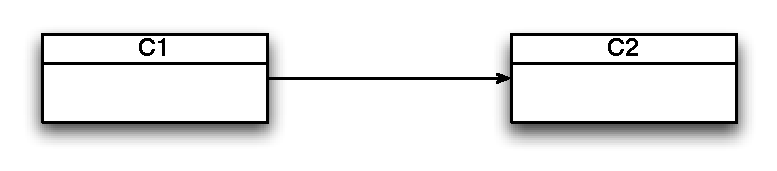
\includegraphics[scale=.5]{fig/delegation.pdf}
    \end{center}
  \end{figure}
  \item La classe cliente (\emph{C1}) utilise les services de la classe serveuse
\end{itemize}
\begin{block}{Schéma type}
\begin{lstlisting}[language=C++]
public class C1 {
private:
   C2 o2; // ou C2 *o2;
\end{lstlisting}
\end{block}
\end{frame}

%%%%%%%%%%%%%%%%%%%%%%%%%%%%%%%%%%%%%%%%%%%%%%
\begin{frame}[fragile]
\frametitle{Délégation : exemple}
\begin{itemize}
  \item Exemple de la classe \emph{Cercle}
  \begin{itemize}
  	\item rayon : un nombre réel
	\item centre : deux réels ou bien un \emph{Point}
  \end{itemize}
\end{itemize}
\begin{lstlisting}[language=C++]
public class Cercle {
private:
  Point centre; // ou Point *centre
  private double rayon;

public:
  Cercle(Point _centre, double _rayon) {
    centre = _centre;
    rayon = _rayon;
  }
};
\end{lstlisting}
\end{frame}

%%%%%%%%%%%%%%%%%%%%%%%%%%%%%%%%%%%%%%%%%%%%%%
\begin{frame}[fragile]
\frametitle{Délégation : exemple}
\begin{itemize}
	\item l'association entre les classes \emph{Cercle} et \emph{Point} exprime le fait qu'un cercle \textbf{possède} (a un) centre
	\item Le point représentant le centre a une existence autonome (cycle de vie indépendant
	\item Il peut être utilisé en dehors du cercle dont il est le centre !
	\begin{itemize}
		\item si on translate le cercle, on translate le point et tous les objets qui utilisent ce point
		\item Solution (en place) : effectuer une copie du point dans le constructeur
	\end{itemize}
\begin{lstlisting}[language=C++]
// cas Point centre
  centre = _centre; // dans les deux cas
// cas Point *centre
  centre = new Point(_centre);
\end{lstlisting}
%% note : les cycles de vie du cercle et du point sont maintenant liés : si le cercle est déplacé ou déruit
%% le point l'est aussi
\end{itemize}
\end{frame}

\subsubsection*{Agrégation / Composition}

%%%%%%%%%%%%%%%%%%%%%%%%%%%%%%%%%%%%%%%%%%%%%%
\begin{frame}{Agrégation / Composition}
\begin{itemize}
	\item L'exemple précédent traduit deux nuances (sémantiques) de l'association \textbf{a un} entre la classe \emph{Cercle} et la classe \emph{Point}
	\item UML distingue deux types de sémantique en définissant deux types de relations
\end{itemize}
\begin{figure}[htbp]
    \begin{center}
      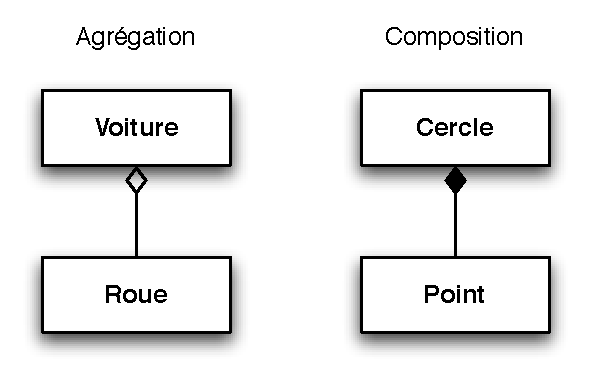
\includegraphics[scale=.45]{fig/agregcompo.pdf}
    \end{center}
  \end{figure}
\end{frame}

%%%%%%%%%%%%%%%%%%%%%%%%%%%%%%%%%%%%%%%%%%%%%%
\begin{frame}{Agrégation / Composition}
\begin{itemize}
	\item \textbf{Agrégation} : l'élément agrégé \emph{Roue} a un existence autonome en dehors de l'agrégat
	\item \textbf{Agrégation forte / composition} : à un même moment, une instance de composant \emph{Point} ne peut être liée qu'à un seul agrégat \emph{Cercle} et le composant a un cycle de vie dépendant de l'agrégat
	\begin{itemize}
	\item Pas vrai dans tous les cas, mais voulu et forcé ici !
	\end{itemize}
\end{itemize}
\end{frame}

\subsubsection*{Syntaxe}

%%%%%%%%%%%%%%%%%%%%%%%%%%%%%%%%%%%%%%%%%%%%%%
\begin{frame}{Héritage : exemple introductif}
\begin{itemize}
	\item Le problème :
	\begin{itemize}
		\item une application a besoin de services dont une partie seulement est proposée par une classe déjà définie
		\item ne pas réécrire le code
	\end{itemize}
\end{itemize}
\begin{figure}[htbp]
    \begin{center}
      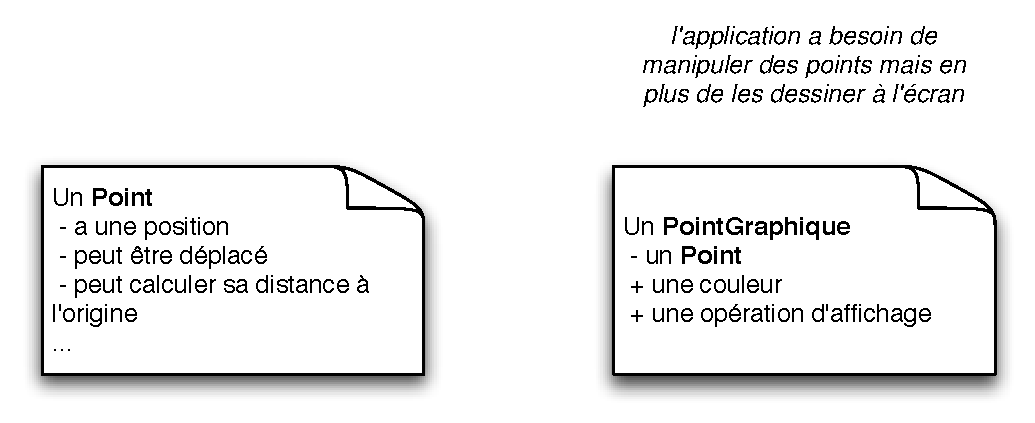
\includegraphics[scale=.42]{fig/pointgraphique.pdf}
    \end{center}
  \end{figure}
\end{frame}

%%%%%%%%%%%%%%%%%%%%%%%%%%%%%%%%%%%%%%%%%%%%%%
\begin{frame}{Pourquoi l'héritage plutôt que agrégation/composition ?}
\begin{itemize}
	\item par simplicité...
	\item ici, on réutilise les méthodes de {Point} dans {PointGraphique}
	\item éviter de rerouter tous les appels à \textit{deplacer()} de {PointGraphique} vers {Point}
	\item exemple opposé : création d'une pile à partir d'une liste
	\begin{itemize}
		\item on ne veut pas donner accès à toutes les méthodes de la liste
	\end{itemize}
\end{itemize}
\end{frame}

%%%%%%%%%%%%%%%%%%%%%%%%%%%%%%%%%%%%%%%%%%%%%%
\begin{frame}[fragile]
\frametitle{Héritage : syntaxe C++}
\begin{itemize}
	\item La classe \emph{PointGraphique} hérite de (elle étend) la classe \emph{Point}
	\begin{itemize}
		\item elle possède les variables et méthodes définies dans la classe \emph{Point} ($x$ et $y$)
		\item elle ajoute des attributs de couleur \texttt{r,g,b}
		\item elle définit une nouvelle méthode \texttt{dessine()}
	\end{itemize}
\end{itemize}
\begin{exampleblock}{Déclaration}
\begin{lstlisting}[language=C++]
class PointGraphique : public Point {
private:
    int r,g,b;

public:
    PointGraphique();
    PointGraphique(double _x,double _y,int _r,int _g, int _b);
    PointGraphique(double _x,double _y);

    void dessine();
};
\end{lstlisting}
\end{exampleblock}
\end{frame}

\begin{frame}[fragile]
\frametitle{Héritage : Ecriture des méthodes}
\begin{itemize}
	\item Seul le constructeur diffère !
	\item Il peut (doit) faire appel au constructeur de la classe \textit{Point}
	\item Syntaxe \texttt{\textit{Pointgraphique::PointGraphique( ) : Point( )}}
\end{itemize}
\begin{exampleblock}{Définition des méthodes}
\begin{lstlisting}[language=C++]
#include "point.h"
#include "pointgraphique.h"

PointGraphique::PointGraphique() : Point() {
    r = g = b = 255; // couleur par defaut = blanc
}

PointGraphique::PointGraphique(double _x,double _y,int _r,int _g, int _b)
 : Point(_x,_y), r(_r), g(_g), b(_b) {
    // plus rien a faire
}

PointGraphique::PointGraphique(double _x,double _y) : Point(_x,_y) {
    r = g = b = 255; // couleur par defaut = blanc
}
\end{lstlisting}
\end{exampleblock}
\end{frame}

%%%%%%%%%%%%%%%%%%%%%%%%%%%%%%%%%%%%%%%%%%%%%%%
\begin{frame}[fragile]
\frametitle{Utilisation des instances d'une classe héritée}
\begin{itemize}
	\item Un objet instance de \emph{PointGraphique} possède les attributs définis dans \emph{PointGraphique} ainsi que ceux définis dans \emph{Point}
	\item Un  objet instance de \emph{PointGraphique} répond aux messages définis par les méthodes décrites dans \emph{PointGraphique} et aussi à ceux définis dans les méthodes de \emph{Point}
\end{itemize}
\begin{exampleblock}{Utilisation}
\begin{lstlisting}[language=C++]
int main() {
    PointGraphique pg;

    pg.setX(5.5);
    pg.setY(2.3);
    pg.translater(2.0, 0.0);
    pg.setCouleur(128, 128, 0);

}
\end{lstlisting}
\end{exampleblock}
\end{frame}

%%%%%%%%%%%%%%%%%%%%%%%%%%%%%%%%%%%%%%%%%%%%%%%
\begin{frame}[fragile]
\frametitle{Résolution statique des messages}
\begin{figure}[htbp]
    \begin{center}
      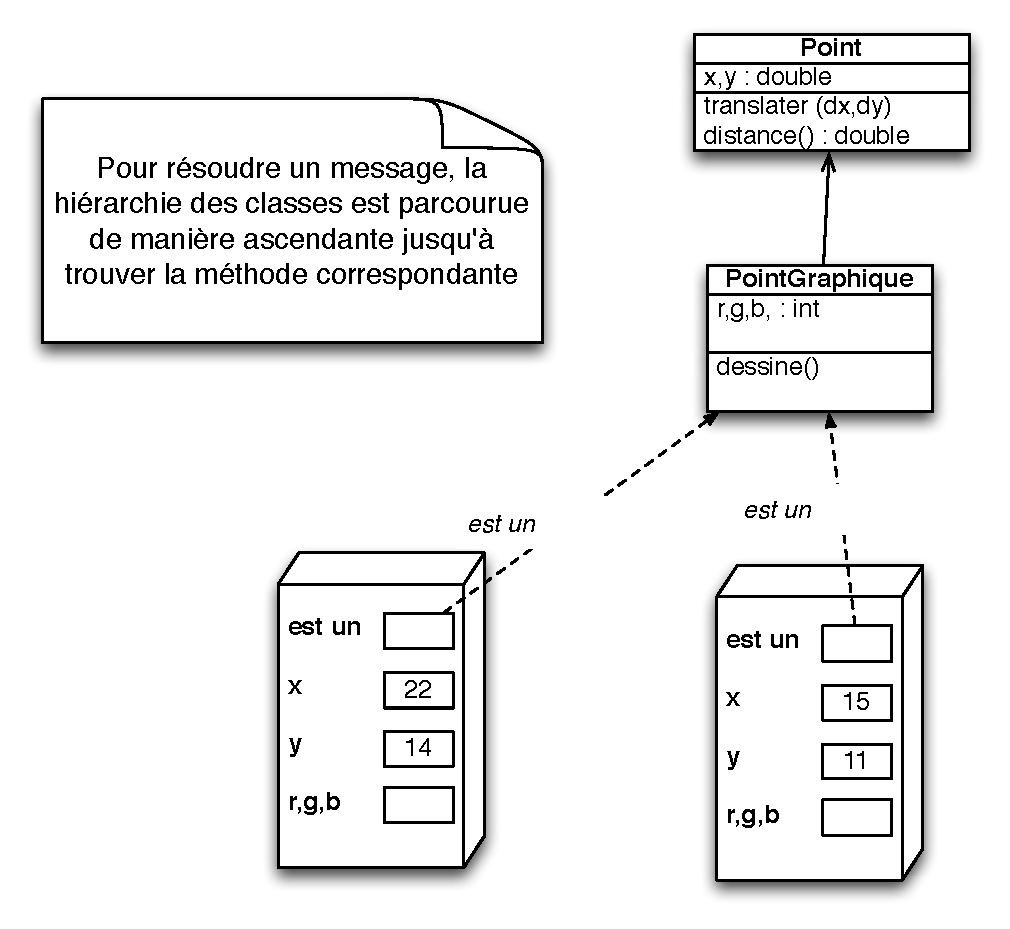
\includegraphics[scale=.42]{fig/resolution.pdf}
    \end{center}
  \end{figure}
\end{frame}

\subsubsection*{Terminologie}

%%%%%%%%%%%%%%%%%%%%%%%%%%%%%%%%%%%%%%%%%%%%%%
\begin{frame}{Terminologie de l'héritage}
\begin{itemize}
	\item L'\textbf{héritage} permet de reprendre les caractéristiques d'une classe $M$ existante pour les étendre et définir ainsi une nouvelle classe $F$ qui hérite de $M$
	\item les objets de $F$ possèdent toutes les caractéristiques de $M$ avec en plus celles définies dans $F$
	\begin{itemize}
		\item $M$ est la classe mère et $F$ la classe fille
		\item $F$ hérite de $M$
		\item $F$ est une sous-classe de $M$
		\item $M$ est la super-classe de $F$
	\end{itemize}
\end{itemize}
\end{frame}

%%%%%%%%%%%%%%%%%%%%%%%%%%%%%%%%%%%%%%%%%%%%%%
\begin{frame}{Généralisation / spécialisation}
\begin{figure}[htbp]
    \begin{center}
      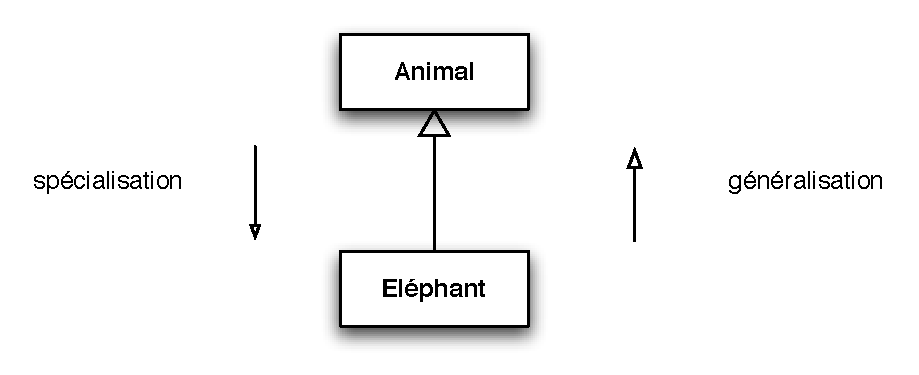
\includegraphics[scale=.45]{fig/genspe.pdf}
    \end{center}
  \end{figure}
\begin{itemize}
	\item la \textbf{généralisation} exprime la relation <<est-un>> entre une classe et sa super-classe
	\item la \textbf{spécialisation} exprime la relation de <<particularisation>> entre une classe et sa sous-classe
\end{itemize}
\end{frame}

%%%%%%%%%%%%%%%%%%%%%%%%%%%%%%%%%%%%%%%%%%%%%%%
\begin{frame}{Généralisation / spécialisation}
\begin{itemize}
	\item Utilisation de la spécialisation : \textbf{réutilisation} par modification incrémentielle des descriptions existantes
	\item Utilisation de la généralisation : \textbf{abstraction} par factorisation des propriétés communes aux sous-classes
	\item il n'y a pas de limitation dans le nombre de niveaux de la hiérarchie d'héritage
	\item les méthodes et les attributs sont automatiquement héritées au travers de tous les niveaux
\end{itemize}
\end{frame}

%\subsection{Redéfinition des méthodes}

%%%%%%%%%%%%%%%%%%%%%%%%%%%%%%%%%%%%%%%%%%%%%%
\begin{frame}{Redéfinition des méthodes}
\begin{itemize}
	\item une sous-classe peut \textbf{redéfinir} des méthodes dont elle hérite et fournir ainsi des implémentations spécialisées pour celles-ci
	\item lorsque la classe définit une méthode dont le nom, le type de retour et les arguments sont identiques à ceux d'une méthode dont on hérite
	\begin{itemize}
	\item On dit aussi qu'une méthode \textbf{masque} celle de la classe mère
	\end{itemize}
	\item Lorsqu'une méthode redéfinie par une classe est invoquée pour un objet de cette classe, c'est la nouvelle définition qui est invoquée
\end{itemize}
\end{frame}

%%%%%%%%%%%%%%%%%%%%%%%%%%%%%%%%%%%%%%%%%%%%%%%
\begin{frame}[fragile]
\frametitle{{\href{code/exheritageA.cxx}{\scalebox{.25}{
\includegraphics{fig/codeicon}}}} Redéfinition des méthodes : exemple (1/2)}
\begin{itemize}
\item Déclaration
\begin{lstlisting}[language=C++]
class exheritageA {
public:
    void hello();
    void affiche();

};

class exheritageB : public exheritageA {
public:
    void affiche();
};
\end{lstlisting}
\item Définition
\begin{lstlisting}
void exheritageA::hello() {
    cout << "hello" << endl;
}

void exheritageA::affiche() {
    cout << "je suis un objet de la classe exheritageA" << endl;
}

void exheritageB::affiche() {
    cout << "je suis un objet de la classe exheritageB" << endl;
}
\end{lstlisting}
\end{itemize}
\end{frame}
%
%%%%%%%%%%%%%%%%%%%%%%%%%%%%%%%%%%%%%%%%%%%%%%%
\begin{frame}[fragile,containsverbatim]
\frametitle{{\href{code/exheritageB.java}{\scalebox{.25}{
\includegraphics{fig/codeicon}}}}  Redéfinition des méthodes : exemple (2/2)}
\begin{lstlisting}[language=C++]
int main() {
    exheritageA a;
    exheritageB b;

    a.hello();
    b.hello();

    a.affiche();
    b.affiche();
}
\end{lstlisting}
\begin{itemize}
	\item produit l'affichage suivant
\end{itemize}
\pause \begin{block}{Résultat}
{\tiny \begin{verbatim}
hello
hello
je suis un objet de la classe exheritageA
je suis un objet de la classe exheritageB
\end{verbatim}}
\end{block}
\end{frame}
%
%
%%%%%%%%%%%%%%%%%%%%%%%%%%%%%%%%%%%%%%%%%%%%%%%
\begin{frame}{Redéfinition des méthodes}
\begin{itemize}
	\item Ne pas confondre redéfinition et surcharge !
\end{itemize}
\begin{figure}[htbp]
    \begin{center}
      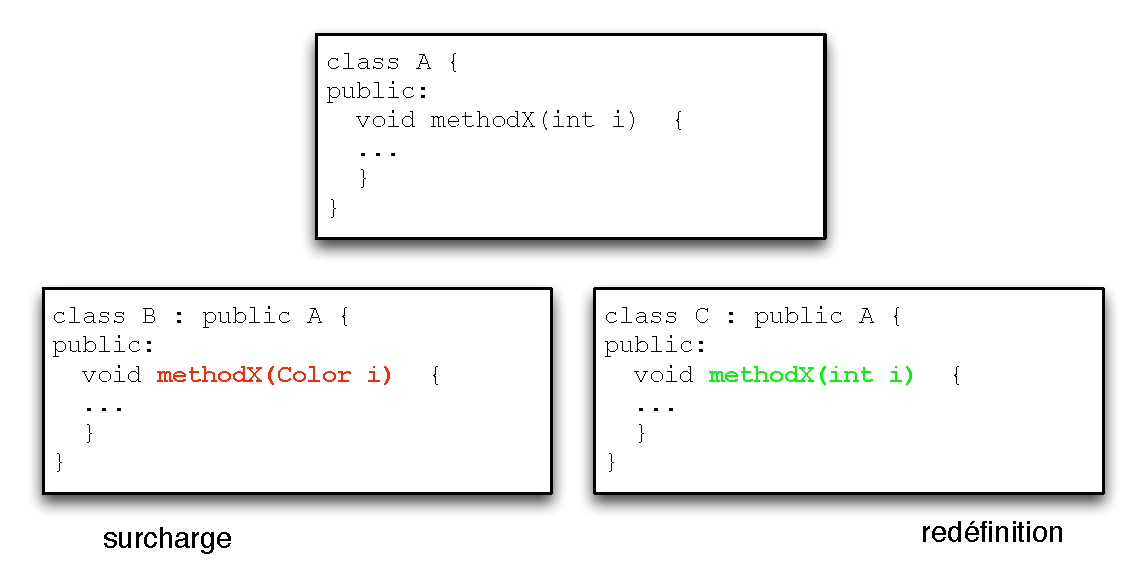
\includegraphics[scale=.45]{fig/rideload.pdf}
    \end{center}
  \end{figure}
\end{frame}

\begin{frame}[fragile]
\frametitle{Limiter les risques (fonctions virtuelles et c+11) !}
  \begin{itemize}
    \item Il arrive qu'on se trompe en redéfinissant une fonction ... ce qui about à une surchage 
    \item Exemple : fonction déclarée dans la classe mère 
  \end{itemize}
  \begin{lstlisting}
    virtual void toto(int a, float b) const ; 
  \end{lstlisting}
  \begin{itemize}
    \item Erreur classique fonction \emph{redéfinie} dans la classe fille 
  \end{itemize}
  \begin{lstlisting}
    virtual void toto(int a, float b) ; 
  \end{lstlisting}
  \begin{itemize}
    \item Solution : le mot clé \texttt{override} dans la déclaration de la classe fille qui annonce qu'il s'agit d'une redéfinition
    \item Le compilateur va vérifier que c'est bien le cas
  \end{itemize}
  \begin{lstlisting}
    virtual void toto(int a, float b) const override; 
  \end{lstlisting}
\end{frame}
%
%%%%%%%%%%%%%%%%%%%%%%%%%%%%%%%%%%%%%%%%%%%%%%%
\begin{frame}[fragile]
\frametitle{{\href{code/heritageC.cxx}{\scalebox{.25}{
\includegraphics{fig/codeicon}}}}  Redéfinition avec réutilisation}
\begin{itemize}
	\item On peut réutiliser le code de la classe mère avec l'opérateur de résolution de portée \texttt{::}
	\item Exemple : Définition d'une classe \textit{exheritageC} similaire à \textit{exheritageB}
\end{itemize}
\begin{lstlisting}[language=C++]
void exheritageC::affiche() {
    exheritageA::affiche();
    cout << "je suis un objet de la classe exheritageC" << endl;
}

// extrait du main()
int main() {
...
    exheritageC c;
    c.affiche();
}
\end{lstlisting}
\pause \begin{block}{Résultat}
{\tiny \begin{verbatim}
je suis un objet de la classe exheritageA
je suis un objet de la classe exheritageC
\end{verbatim}}
\end{block}
\end{frame}

\subsubsection{Retour sur les protections}

\begin{frame}{Protection}

\begin{itemize}
\itemsep1pt\parskip0pt\parsep0pt
\item
  Situation actuelle

  \begin{itemize}
  \itemsep1pt\parskip0pt\parsep0pt
  \item
    \textbf{public} accessible depuis partout (sous réserve de disposer
    d'une instance de la classe)
  \item
    \textbf{private} accessible uniquement depuis l'intérieur (i.e.~les
    méthodes de la classe)
  \item
    problème : une classe dérivée ne peut accéder aux membres privés de
    sa classe mère
  \end{itemize}
\item
  Solution

  \begin{itemize}
  \itemsep1pt\parskip0pt\parsep0pt
  \item
    \textbf{protected} : accessible depuis l'intérieur de la classe et
    de toutes les classes dérivées
  \end{itemize}
\item
  Ce n'est pas tout

  \begin{itemize}
  \itemsep1pt\parskip0pt\parsep0pt
  \item
    notion de fonctions \textbf{friend}
  \item
    héritage via le mot-clé \textbf{public}\ldots{} il existe d'autres
    formes d'héritage
  \item
    classes internes
  \end{itemize}
\end{itemize}

\end{frame}

\subsubsection{Exemple}

\begin{frame}{Exemple : compte bancaire avec autorisation de découvert}
\begin{itemize}
\item Compte bancaire "standard" : notion forcément incomplète
\begin{itemize}
\item en pas uniquement en raison de nos simplifications
\end{itemize}
\item On peut avoir différents types de comptes bancaires
\item Exemple : certains comptes ont une autorisation de découvert, c'est-à-dire qu'on peut avoir un \textit{solde légèrement négatif}, dans une limite fixée par la banque
\item Nouvel attribut
\begin{itemize}
\item le montant du découvert autorisé
\end{itemize}
\item Méthodes
\begin{itemize}
\item modification de la méthode \textit{debiter()}
\item ajout d'un setter pour le montant du découvert autorisé
\item le reste est identique
\end{itemize}
\end{itemize}
\end{frame}

\begin{frame}[fragile]\frametitle{Exemple : le code (1/2)}
\begin{codeblock}{Déclaration de la classe}
\begin{lstlisting}
class comptead : public compte {
protected:
    float montant_ad;

public:
    bool debiter(float montant);
    void infos() const;
    void setMontantAD(float m);
    comptead(int numero);
};
\end{lstlisting}
\end{codeblock}
\end{frame}


\begin{frame}[fragile]\frametitle{Exemple : le code (2/2)}
\begin{codeblock}{Définition des méthodes}
\begin{lstlisting}
void comptead::setMontantAD(float m) {
    montant_ad = m;
}


bool comptead::debiter(float montant) {
    if (!ib && solde+montant_ad>=montant) {
        solde -= montant;
        return true;
    }
    return false;
}

comptead::comptead(int n) : compte(n) {
    montant_ad = 0.0;
}

void comptead::infos() const {
    compte::infos();
    cout << "montant de l'autorisation de decouvert : " << montant_ad << endl;
}
\end{lstlisting}
\end{codeblock}

\end{frame}
%\subsubsection{Héritage multiple}
